\chapter{控制系统的性能指标}
\label{chap:performance-metrics}

\section{稳定裕度}

关于稳定裕度的部分，详情请见系统稳定性与分析中的\hyperref[sec:stability-margin]{稳定裕度}这一节，本章不再复述其定义，只谈其应用。

以下部分均以二阶系统为例进行讨论：

\subsection{二阶系统的稳定裕度}

在经典二阶单位反馈系统（如下图）中，我们可以写出其开环传递函数为：
\begin{center}
    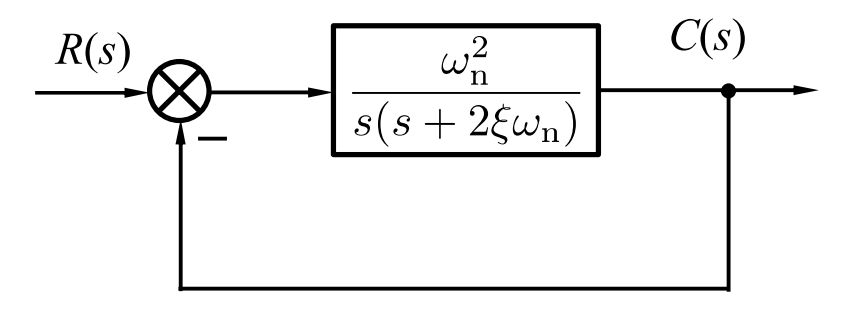
\includegraphics[width=.5\textwidth]{note/performance metrics/figure/1.png}
\end{center}
\begin{equation*}
    G(s) = \frac{\omega_n^2}{s^2 + 2 \omega_n \xi s}
\end{equation*}

故由剪切频率的定义可知：$\omega_c = \omega_n \sqrt{{\sqrt{4 \xi^4 + 1} - 2\xi^2}}$

其相角裕度为：$\gamma = 90\text{°} - \arctan{\dfrac{\sqrt{\sqrt{4 \xi^4 + 1} - 2\xi^2}}{2 \xi}}$

由于其穿越频率$\omega_g = \infty$，故其相位裕度$K_g = \infty$

\section{闭环频域的性能指标}
对于一个一般的系统，我们可以给出其广义的示意图如下：
\begin{center}
    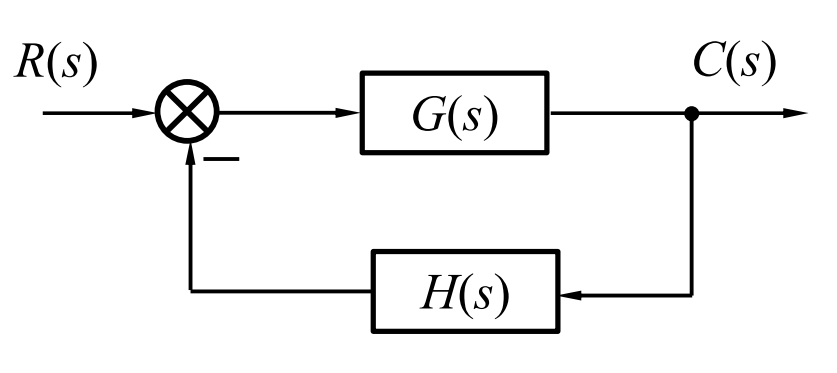
\includegraphics[width=.5\textwidth]{note/performance metrics/figure/2.png}
\end{center}

根据上图，我们可以给出其前向通路和反馈通路的表达式如下：
\begin{enumerate}
    \item 前向通路：$G(s) = \dfrac{K G_1(s)}{s^v}$
    \item 反馈通路：$H(s) = K_h H_1(s)$
\end{enumerate}

其中$K$为前向通路增益，$K_h$为反馈通路的增益，$G_1(s)$和$H_1(s)$在0处均有值为1。

所以闭环传递函数的频域幅值为：
\begin{equation*}
    \begin{split}
        A(\omega) &= \left\lvert \frac{G(j\omega)}{1 + G(j\omega) H(j\omega)} \right\rvert     \\
        &=\frac{\left\lvert K G_1(j\omega)\right\rvert}{\left\lvert (j\omega)^v + K K_h G_1(j\omega) H_1(j\omega)\right\rvert }
    \end{split}
\end{equation*}

根据上面的式子我们可以得到幅值在0处的值为：
\begin{equation*}
    A(0) = 
    \begin{cases}
        \frac{1}{K_h} & v\geq 1 \\
        \frac{K}{1 + K K_h} & v = 0\\ 
    \end{cases}
\end{equation*}

故$1-A(0)$为单位阶跃响应的稳态误差



\textbf{闭环频域的性能指标一共有以下几个：}
\begin{enumerate}
    \item 零频幅值：即$A(0)$
    \item 相对谐振峰值：$M_r = \dfrac{\max A(\omega)}{A(0)}$
    \item 谐振频率：出现谐振峰值时的频率，其满足$A(\omega_r) = \max_{\omega} A(\omega)$
    \item 截止频率：幅值下降到零频幅值的$\frac{\sqrt{2}}{2}$时的频率，即 $A(\omega_b) = \frac{\sqrt{2}}{2} A(0)$
\end{enumerate}

\subsection{二阶系统的闭环频域性能}
对于一个经典二阶系统（如下图所示）我们可以给出其闭环频率特性和幅频特性：
\begin{center}
    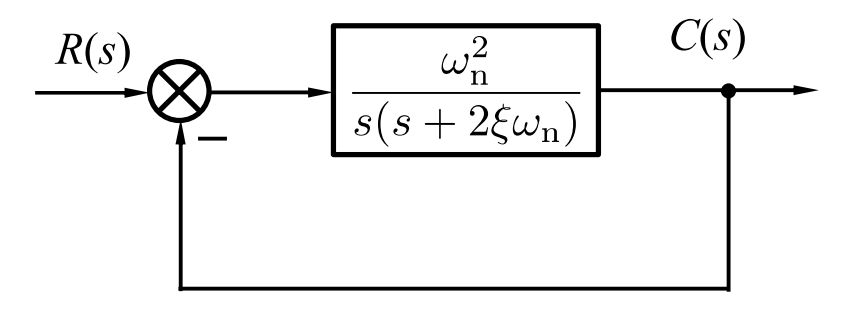
\includegraphics[width = .5\textwidth]{note/performance metrics/figure/1.png}
\end{center}
\begin{equation*}
    \begin{split}
        \Phi(j \omega) &= \frac{\omega_n^2}{(j\omega)^2 + 2j\xi \omega_n \omega + \omega_n^2} \\
        A(\omega) &= \left\lvert \Phi(j\omega) \right\rvert = \frac{\omega_n^2}{\sqrt{(\omega_n^2 - \omega^2)^2 + 4 \xi^2 \omega_n^2 \omega^2}}\\
    \end{split}
\end{equation*}

同时我们可以给出闭环幅频特性曲线如下：
\begin{center}
    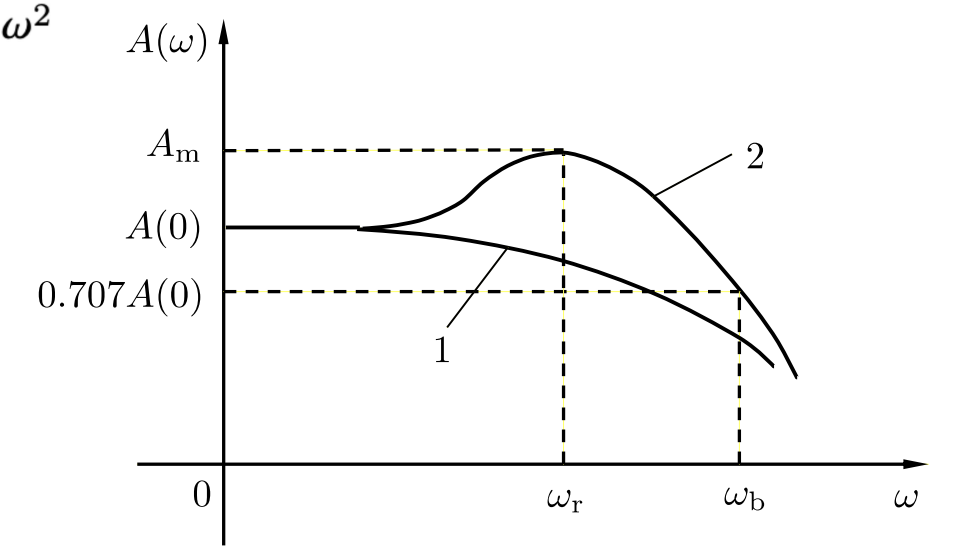
\includegraphics[width = .5\textwidth]{note/performance metrics/figure/3.png}
\end{center}

由图和式子可以知道谐振频率$\omega_r = \omega_n \sqrt{1-2 \xi^2}$，相对谐振峰值$M_r = \frac{1}{2 \xi \sqrt{1-\xi^2}}$

同样的，根据截止频率的定义我们也可以得到谐振频率的式子为：$\omega_b = \omega_n \sqrt{1-2\xi^2 + \sqrt{2 - 4\xi^2 + 4\xi^4}}$

\subsection{闭环特性的图示法：等M圆}
设系统为单位负反馈系统，设开环传递函数$G(j \omega) = U + jV$，闭环传递函数的幅值为$M$，则有：
\begin{equation*}
    (U + \frac{M^2}{M^2 - 1})^2 + V^2 = \frac{M^2}{(M^2 - 1)^2}
\end{equation*}

由式子可知，这是一个关于开环传递函数实部和虚部的一个圆，圆的圆心和半径由闭环频率特性的幅值确定，等M圆示意图如下：
\begin{center}
    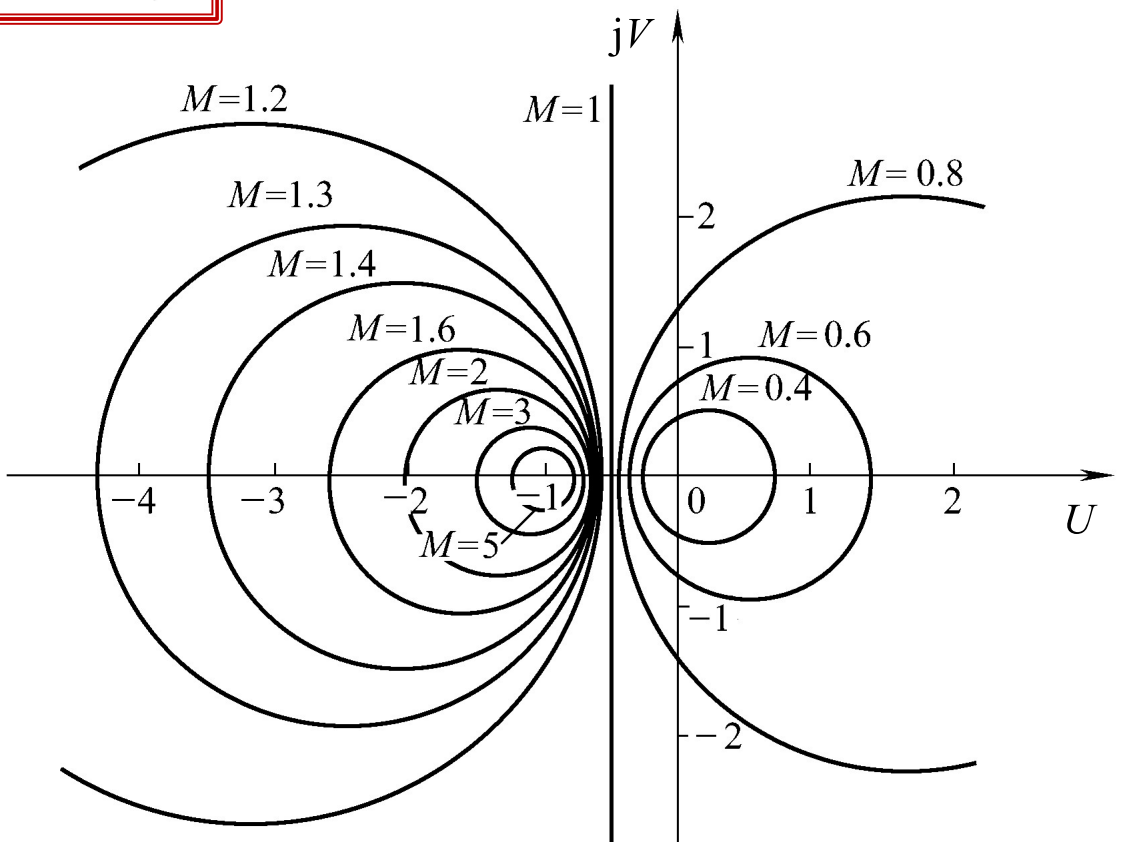
\includegraphics[width = .5\textwidth]{note/performance metrics/figure/4.png}
\end{center}

由图和式子我们可以得到：
\begin{enumerate}
    \item $M > 1$时，圆心在虚轴左侧，且半径随$M$的增大而减小，当$M \to \infty$时圆心在(-1,0)处
    \item $M < 1$时，圆心在虚轴的右侧，且半径随$M$的增大而增大，当$M \to 0$时圆心在(0,0)处
    \item $M = 1$时，圆退化为直线$U = -\frac{1}{2}$
\end{enumerate}

等M圆的具体用法如下：

我们可以在等M圆图里画出系统的Nyquist曲线，根据曲线和等M圆的相交的情况可以确定系统的闭环幅频特性曲线，当Nyquist曲线与某一M圆相切时，相切M圆的M值就是闭环幅频特性的谐振峰值$M_r$，切点处的$\omega$就是谐振频率$\omega_r$

\section{不同域下性能指标的关系}

\subsection{闭环频域指标和开环频域指标之间的关系}

对于单位反馈系统，如果$G(s)$是I型或以上系统，则有$A(0) = 1$；如果$G(s)$是0型系统，且其开环增益较高，则有$A(0) \approx 1$。则有以下式子成立：
\begin{equation*}
    M_r = \frac{A_{max}}{A(0)} \approx \frac{1}{\sin \gamma}
\end{equation*}
或者
\begin{equation*}
    \gamma = \arcsin \frac{1}{M_r}
\end{equation*}
根据以上两个式子，以及7.1.1中的$w_c$和$\gamma$，和7.2.1中的$M_r$，$\omega_r$，$\omega_b$我们可以得到经典二阶系统中的闭环频域指标和开环频域指标的关系为：
\begin{center}
    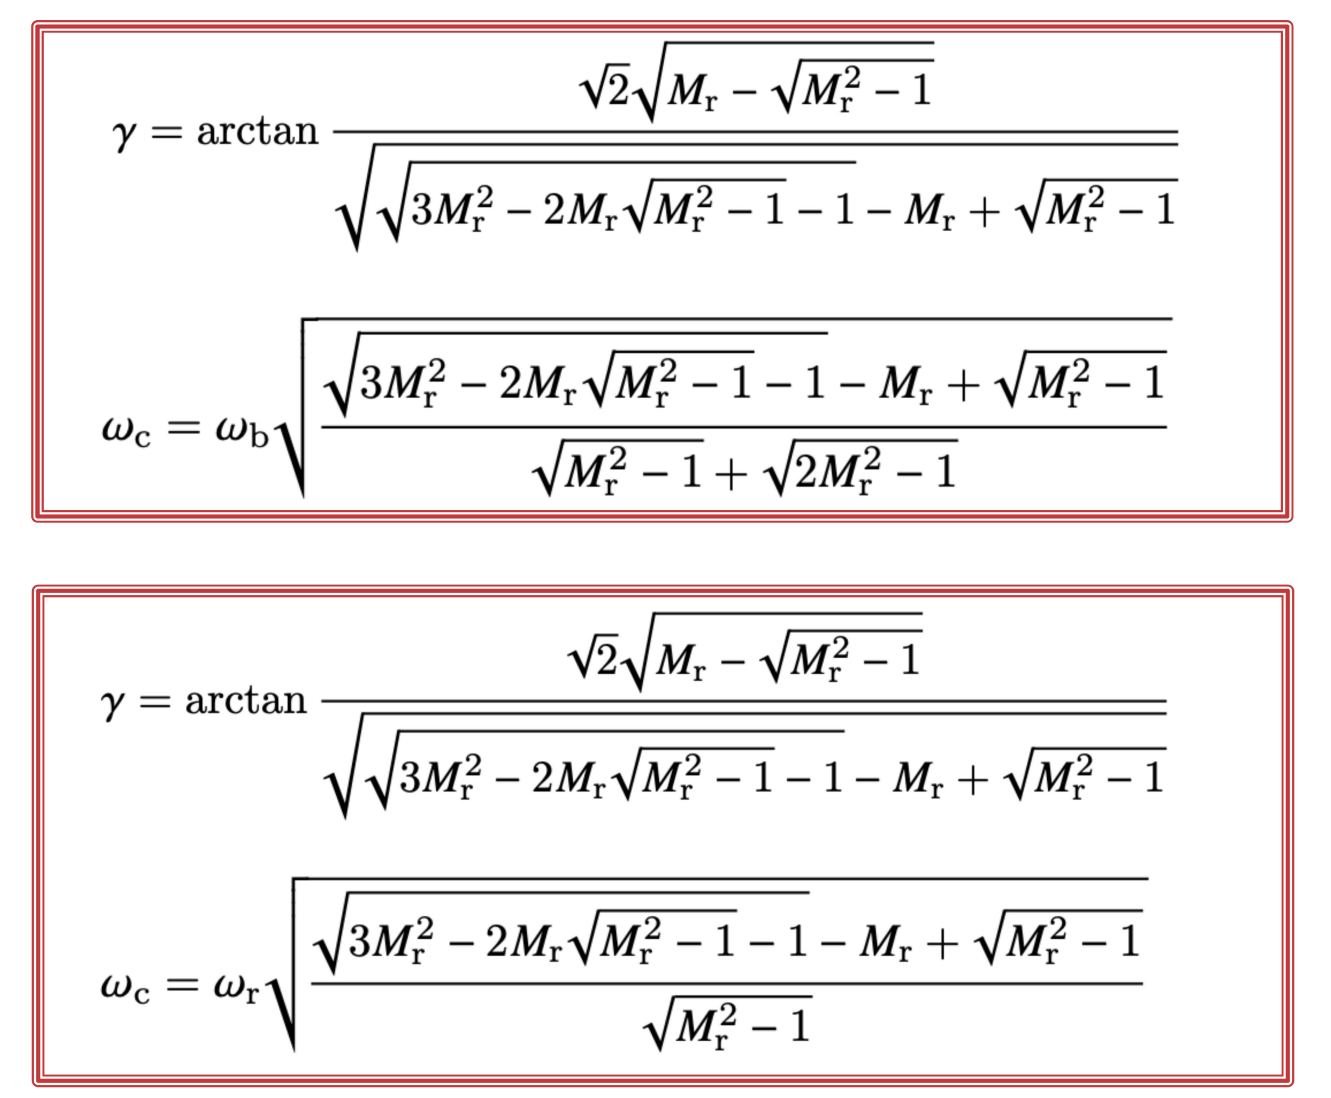
\includegraphics[width = .7\textwidth]{note/performance metrics/figure/5.png}
\end{center}

\subsection{闭环频域指标和时域指标之间的关系}

在经典二阶系统时域中，我们有以下几个指标：
\begin{enumerate}
    \item $\sigma_p = \text{exp}\left( \frac{-\xi \pi}{\sqrt{1- \xi^2 }}\right)$
    \item $t_s = \frac{4}{\xi \omega_n} \quad \Delta = 0.05$
    \item $t_p = \frac{\pi}{\omega_n \sqrt{1 - \xi^2}}$
\end{enumerate}

再根据7.1.1中的$w_c$和$\gamma$，和7.2.1中的$M_r$，$\omega_r$，$\omega_b$我们可以得到经典二阶系统中的闭环频域指标和时域指标的关系为：

\begin{center}
    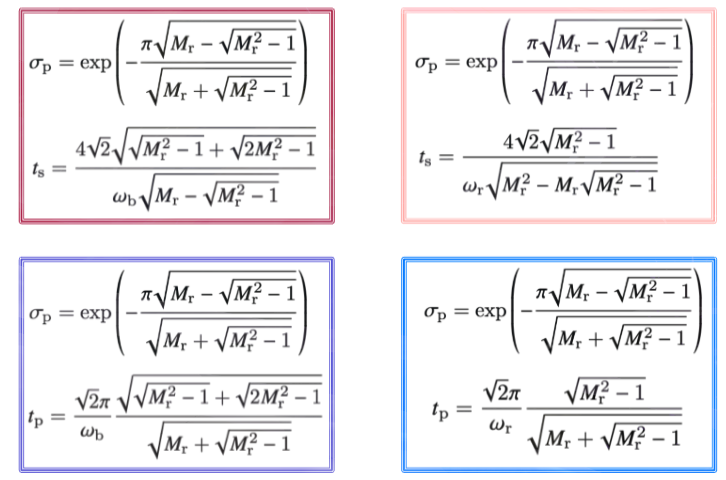
\includegraphics[width = .6\textwidth]{note/performance metrics/figure/6.png}
\end{center}

由于这上面几组式子太难算了，前人在此基础上得到了经验公式：

\begin{center}
    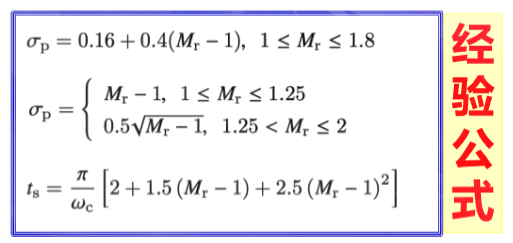
\includegraphics[width = .6\textwidth]{note/performance metrics/figure/7.png}
\end{center}

\subsection{开环频域指标和时域指标之间的关系}

由上面的式子可以知道有以下几组式子成立：
\begin{equation*}
    \begin{split}
        \sigma_p &= \text{exp}\left( \frac{-\pi}{\sqrt{2 \sqrt{M^2 - 1} - 1}} \right) \\
        M &= \frac{2 + \tan^2 \gamma}{\tan^2 \gamma} \\
        \omega_c t_p &= \frac{2\pi}{\tan \gamma} \frac{1}{\sqrt{ 2 \sqrt{M^2 - 1} - 1}}\\
        t_s &= \frac{8}{\omega_c \tan \gamma}
    \end{split}
\end{equation*}

同样的，在这组式子的基础上前人也总结出了一组经验公式：
\begin{center}
    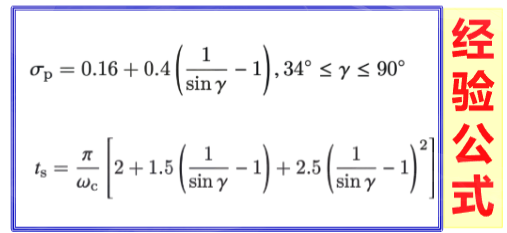
\includegraphics[width = .6\textwidth]{note/performance metrics/figure/8.png}
\end{center}

\section{三频段理论}

\subsection{三频段的划分}
根据Bode中的频率与剪切频率，转折频率等特殊频率之间的关系我们可以将Bode图划分为以下图中的三段：
\begin{center}
    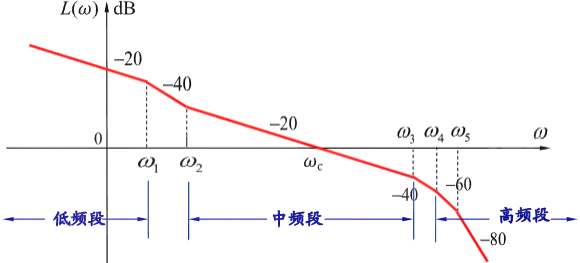
\includegraphics[width = .5\textwidth]{note/performance metrics/figure/9.png}
\end{center}
\begin{enumerate}
    \item 低频段：第一个转折频率之前的频段
    \item 中频段：剪切频率附近的频段，一般为剪切频率前一个转折频率到剪切频率后一个转折频率之间的频段
    \item 高频段：通常为中频段之后的频段，一般为$\omega > 10 \omega_c$的频段，其中$\omega_c$为剪切频率，这部分特性是由系统中小时间常数的环节决定的，由于远离剪切频率，一般分贝值又比较低，故对系统的动态响应影响不大

    在高频段，由于系统的开环幅频特性$G(j\omega)$远小于1，因此对单位负担亏系统有：
    \begin{equation*}
        \left\lvert \Phi(j\omega) \right\rvert = \left\lvert \frac{G(j\omega)}{1 + G(j\omega)} \right\rvert \approx \left\lvert G(j\omega) \right\rvert 
    \end{equation*}
    故在高频段，开环与闭环对数幅频特性近似相等，直接反映了系统抑制输入端高频干扰的能力。高频段的分贝值越低，系统的抗干扰能力就越强
\end{enumerate}

\subsection{两类特殊的中频段}
下面我们将讨论中频段斜率分别为-20dB/dec和-40dB/sec时的特性
\begin{enumerate}
    \item 中频段斜率为-20dB/sec时：\\
          此时这一段的开环传递函数和闭环传递函数可以近似为：
          \begin{equation*}
            \begin{split}
                G(s) &= \frac{K}{s} \\
                \Phi(s) &= \frac{K}{s + K} = \frac{1}{\frac{s}{K} + 1}               
            \end{split}
          \end{equation*}
          此时系统非常容易稳定
    \item 中频段斜率为-40dB/sec时：\\
          此时这一段的开环传递函数和闭环传递函数可以近似为：
          \begin{equation*}
            \begin{split}
                G(s) &= \frac{K}{s^2} \\
                \Phi(s) &= \frac{K}{s^2 + K} = \frac{\omega_c^2}{s^2 + \omega_c^2}
            \end{split}
          \end{equation*}
\end{enumerate}

\subsection{一个设计合理的系统的三频段的要求}
对于一个设计合理的系统的三频段，我们有以下的要求:
\begin{enumerate}
    \item 中频段的斜率以-20dB/sec为宜
    \item 低频段和高频段可以有更大的斜率，低频段的斜率越大，系统的稳态性能越强，高频段的斜率越大，系统排除干扰的能力越强
    \item 中频段必须有足够的带宽，以保证系统的相位裕量，带宽越大，相位裕量越大；$\omega_c$的大小也很重要，$\omega_c$越大系统的快速性越好，但是抗干扰的能力会下降
\end{enumerate}

\subsection{低频段和高频段的斜率对中频段剪切频率的影响}

\subsubsection{低频段对中频段剪切频率的影响}

\begin{center}
    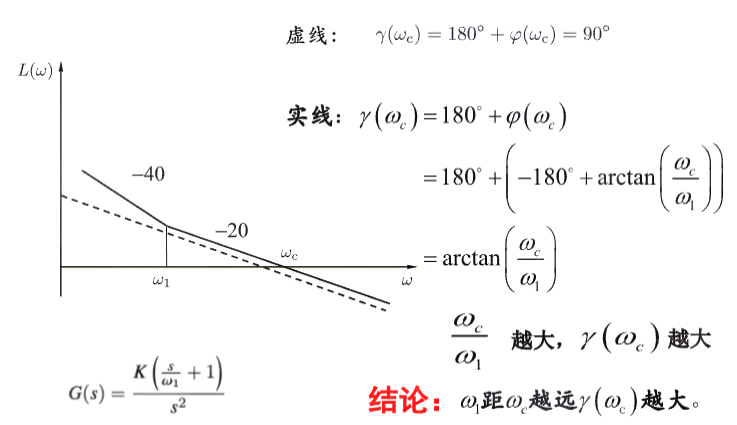
\includegraphics[width = .8\textwidth]{note/performance metrics/figure/10.png}
\end{center}

\subsubsection{高频段对中频段剪切频率的影响}

\begin{center}
    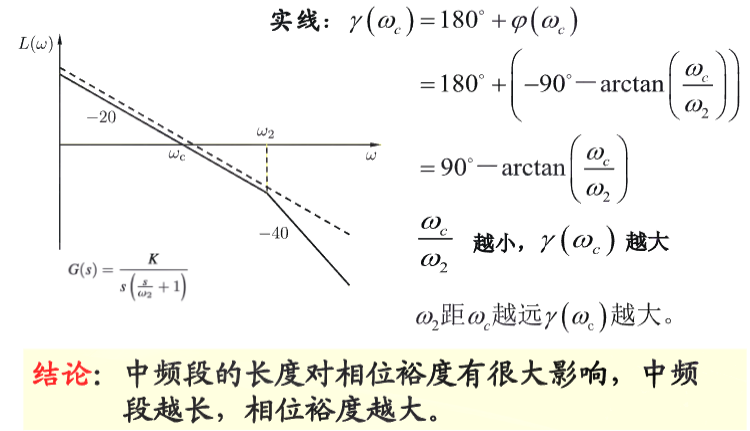
\includegraphics[width = .8\textwidth]{note/performance metrics/figure/11.png}
\end{center}

\subsection{开环增益变化对相位裕度的影响}

\begin{center}
    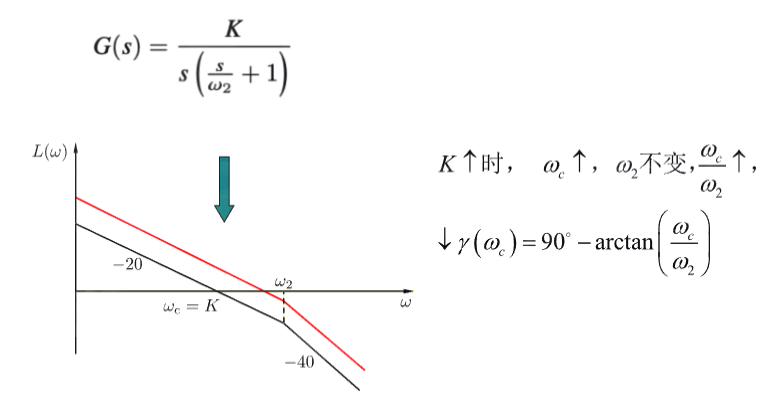
\includegraphics[width = .8\textwidth]{note/performance metrics/figure/12.png}

    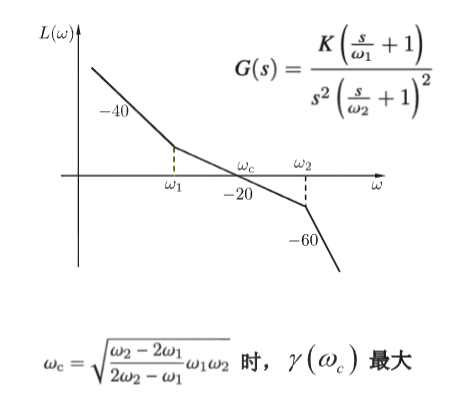
\includegraphics[width = .4\textwidth]{note/performance metrics/figure/13.png}

    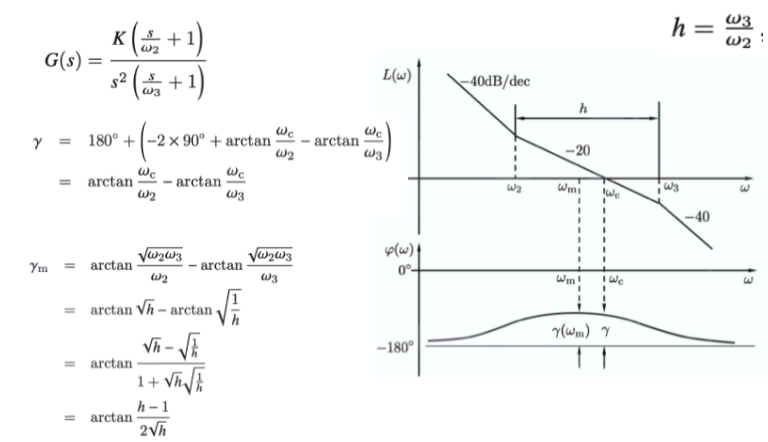
\includegraphics[width = .6\textwidth]{note/performance metrics/figure/14.png}
\end{center}
